\documentclass{article}
\usepackage{graphicx} % Required for inserting images

\title{Problem Set 8}
\author{Krishna Dindial }
\date{https://github.com/kdindial/phys-ga2000}

\begin{document}

\maketitle

\section{Problem 1}
\begin{figure}
    \centering
    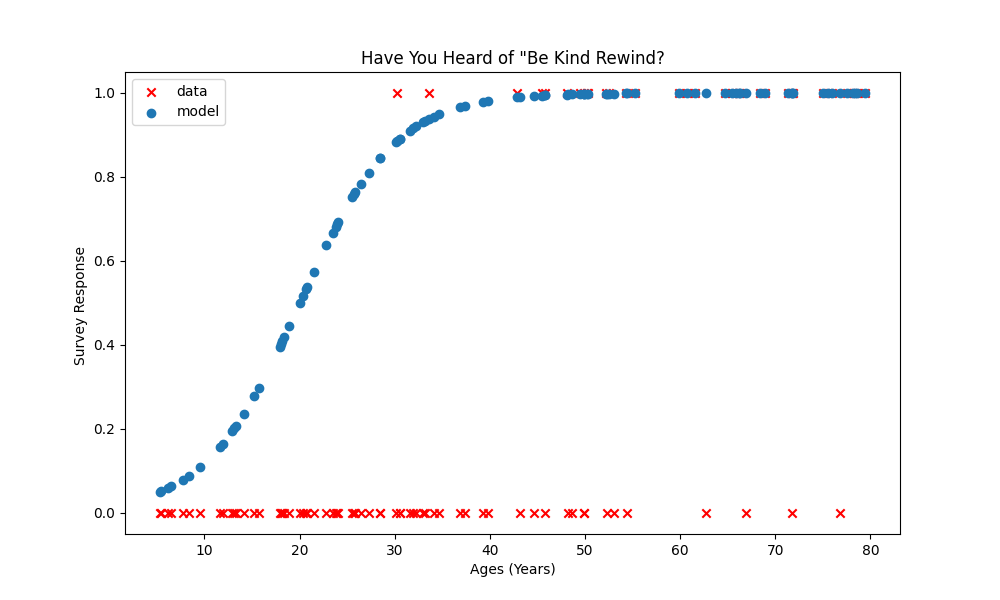
\includegraphics[width=\linewidth]{fit.png}
    \caption{Survey Response Logistical Fit}
    \label{fig:enter-label}
\end{figure}


The values of b0 and b1 that I found maximize the likelihood, were b0=0.9308 and b1=0.01878. This means that people who are 50 years old have about a 50 percent chance of having heard about be kind rewind. This seems a bit old to me, but based off the data it seems like there were a fair amount of people above 50 who had never heard of it. \par
The covariance matrix I found was:

\begin{equation}
    \begin{array}{cc}
       8.6655641e-01  &-1.6613813e-02\\
      -1.6613811e-02   & 3.5285315e-04

    \end{array}
\end{equation}

The formal errors for b0 was very high. It was 93 percent. For b1 it was 18 percent. It makes sense that the error for b0 would be high because the ratio of b1/b0 determines the age at which there is a 5050 percent chance the person had heard of "bkr" because there is a wide overlap of young people who have heard of it and old people who havent heard of it. Fig 1 shows the plot of the data with the logistic regression model over it.


\section{Problem 2}

 Figures 2 and 3 show the wave form of the trumpet and the piano. Figure 4 shows  the  frequency spectrum of the two instruments. The piano spectrum is mostly dominated by the fundamental frequency at around 262Hz. Overall it has much less harmonic content than the trumpet. The piano spectrum has a small bump in the around 0Hz. This is from percussive sound of striking of the piano key. You can see this in the waveform of the piano because it starts with a spike then settles to something more sinusoidal. The harmonics of the trumpet are much more dominant in its spectrum. \par
 The way that I tried to find the notes that each instrument was playing, was to take the Fourier coefficient that had the highest amplitude and say that was the note it was playing, but the coefficient of the trumpet that has the highest amplitude is actually the second fundamental, as you can see from figure 4. The way I found the note the trumpet was playing was by finding the frequency with the largest coefficient below 400Hz. I found that the piano was playing 260.4105Hz and the trumpet was playing 262.6155 Hz.

 \begin{figure}
     \centering
     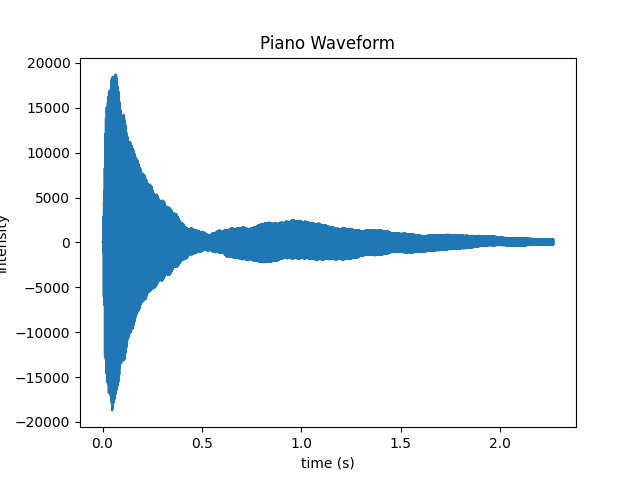
\includegraphics[width=\linewidth]{piano.png}
     \caption{Piano Waveform}
     \label{fig:enter-label}
 \end{figure}

 \begin{figure}
     \centering
     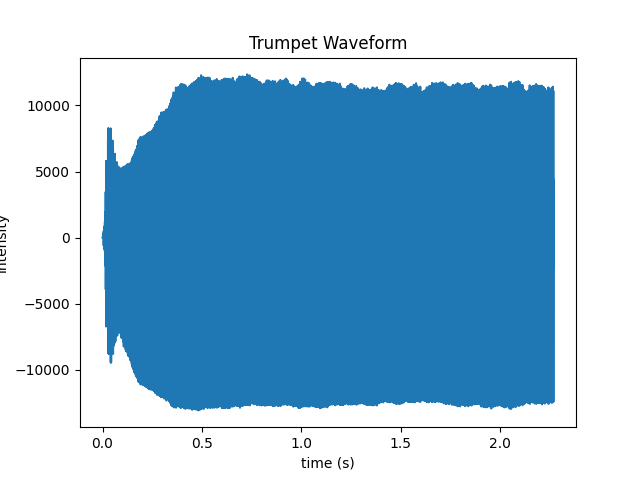
\includegraphics[width=\linewidth]{trumpet.png}
     \caption{Trumpet Waveform}
     \label{fig:enter-label}
 \end{figure}

\begin{figure}
    \centering
    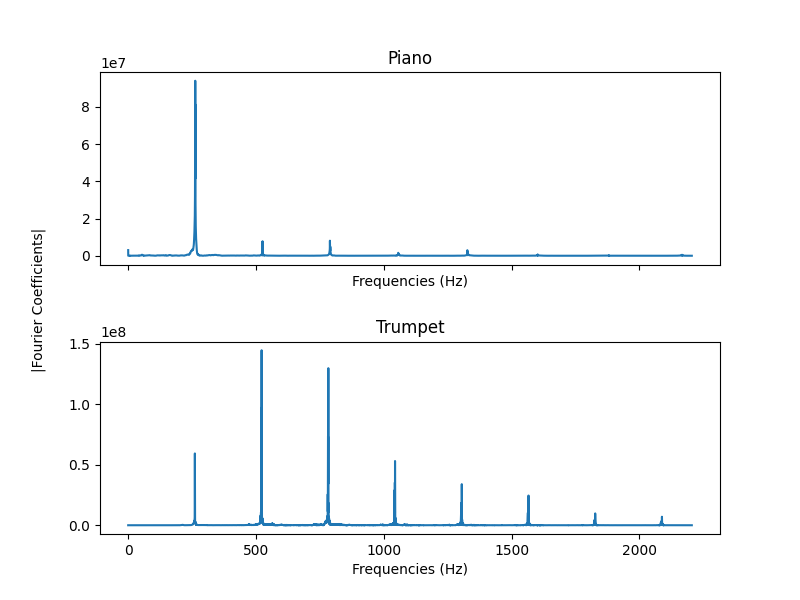
\includegraphics[width=\linewidth]{problem2.png}
    \caption{Spectrum of Piano and Trumpet}
    \label{fig:enter-label}
\end{figure}
\section{Problem 3}

Figure 5 shows the unfiltered DJI, and figure 6 shows the DJI inverse fft that only keeps the fist 10 percent of coefficients and the dow inverse fft that only keeps the first 2 percent of the coefficients overlayed




\begin{figure}
    \centering
    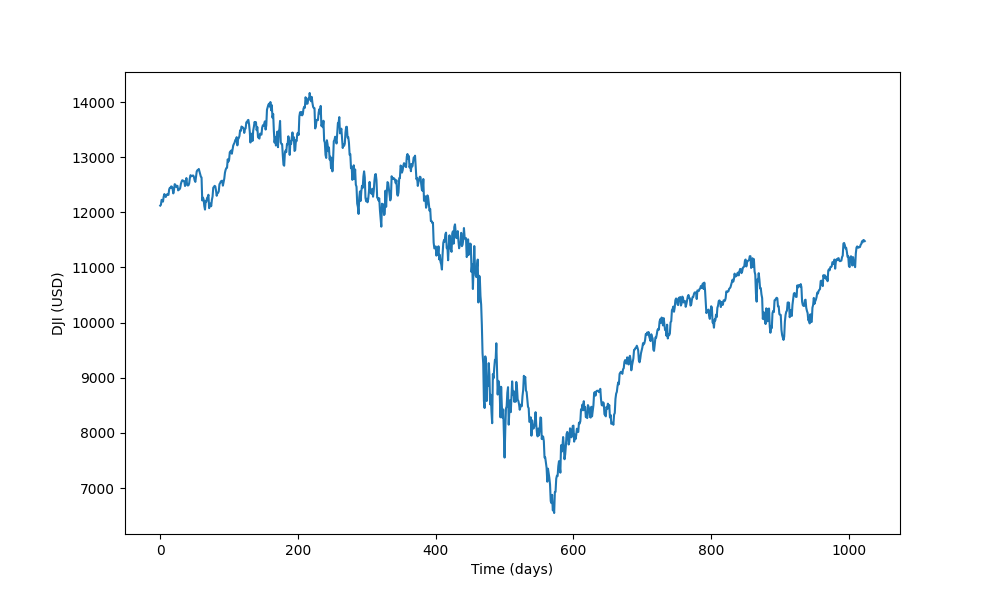
\includegraphics[width=\linewidth]{dow.png}
    \caption{Dow}
    \label{fig:enter-label}
\end{figure}

\begin{figure}
    \centering
    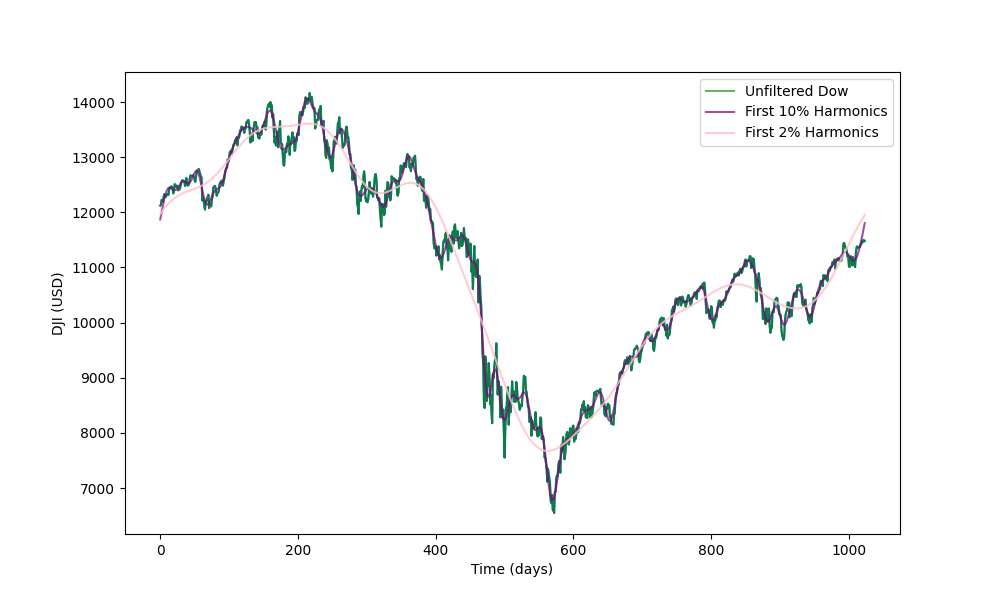
\includegraphics[width=\linewidth]{dow_10.png}
    \caption{Filtered Dow}
    \label{fig:enter-label}
\end{figure}
\end{document}
